\documentclass{scrartcl}

% Packages
% ---
\usepackage[export]{adjustbox}
\usepackage[utf8]{inputenc} % Unicode support (Umlauts etc.)
\usepackage{amsmath}
\usepackage{cprotect} % Allow verbatim text in macro arguments
\usepackage{dirtytalk} % For proper quotations
\usepackage{graphicx} % Add pictures to your document
\usepackage{hyperref} % Add a link to your document
\usepackage{minted} % Source code formatting and highlighting
\usepackage{wrapfig}
\usepackage{xcolor}
\usepackage{lmodern}
\usepackage[T1]{fontenc}

\numberwithin{figure}{subsection}
\graphicspath{{img/}}

\setlength{\parindent}{0em}
\setlength{\parskip}{1em}

\definecolor{beige}{rgb}{0.95,0.95,0.92}
\hypersetup{
    pdfborderstyle={/S/U/W 1},
    pdfauthor=Christophe Riccio,
    pdftitle=GLM Manual
}

\usemintedstyle{borland}
\newminted{cpp}{linenos, bgcolor=beige}
\newminted{glsl}{linenos, bgcolor=beige}


\begin{document}

\newcommand{\glmheader}[1]{\href{https://github.com/g-truc/glm/tree/master/glm/#1.hpp}{\texttt{<glm/#1.hpp>}}}
\newcommand{\glmemail}[1]{\href{mailto://glm@g-truc.net}{#1}}
\newcommand{\glufunction}[1]{\href{https://www.opengl.org/sdk/docs/man2/xhtml/#1.xml}{\texttt{#1}}}
\newcommand{\glfunction}[2]{\href{http://docs.gl/gl#1/#2}{\texttt{#2}}}

% Set up the maketitle command
\author{Christophe Riccio}
\subtitle{Version 0.9.7}

\title{GLM Manual}
\date{\today{}} % You can remove \today{} and type a date manually

\maketitle{} % Generates title

\pagebreak{}

\section*{Licensing}
\addcontentsline{toc}{section}{Licensing}

\subsection*{\hypertarget{happybunny}{The Happy Bunny License (Modified MIT License)}}
\addcontentsline{toc}{subsection}{The Happy Bunny License (Modified MIT License)}

\copyright{} 2008 - 2015 G-Truc Creation

Permission is hereby granted, free of charge, to any person obtaining a copy of this software and associated documentation files (the \say{Software}), to deal in the Software without restriction, including without limitation the rights to use, copy, modify, merge, publish, distribute, sublicense, and/or sell copies of the Software, and to permit persons to whom the Software is furnished to do so, subject to the following conditions:

The above copyright notice and this permission notice shall be included in all copies or substantial portions of the Software.

Restrictions: By making use of the Software for military purposes, you choose to make a Bunny unhappy.

THE SOFTWARE IS PROVIDED \say{AS IS}, WITHOUT WARRANTY OF ANY KIND, EXPRESS OR IMPLIED, INCLUDING BUT NOT LIMITED TO THE WARRANTIES OF MERCHANTABILITY, FITNESS FOR A PARTICULAR PURPOSE AND NONINFRINGEMENT. IN NO EVENT SHALL THE AUTHORS OR COPYRIGHT HOLDERS BE LIABLE FOR ANY CLAIM, DAMAGES OR OTHER LIABILITY, WHETHER IN AN ACTION OF CONTRACT, TORT OR OTHERWISE, ARISING FROM, OUT OF OR IN CONNECTION WITH THE SOFTWARE OR THE USE OR OTHER DEALINGS IN THE SOFTWARE.

\pagebreak{}

\subsection*{\hypertarget{mit}{The MIT License}}
\addcontentsline{toc}{subsection}{The MIT License}

\copyright{} 2008 - 2015 G-Truc Creation

Permission is hereby granted, free of charge, to any person obtaining a copy of this software and associated documentation files (the \say{Software}), to deal in the Software without restriction, including without limitation the rights to use, copy, modify, merge, publish, distribute, sublicense, and/or sell copies of the Software, and to permit persons to whom the Software is furnished to do so, subject to the following conditions:

The above copyright notice and this permission notice shall be included in all copies or substantial portions of the Software.

THE SOFTWARE IS PROVIDED \say{AS IS}, WITHOUT WARRANTY OF ANY KIND, EXPRESS OR IMPLIED, INCLUDING BUT NOT LIMITED TO THE WARRANTIES OF MERCHANTABILITY, FITNESS FOR A PARTICULAR PURPOSE AND NONINFRINGEMENT. IN NO EVENT SHALL THE AUTHORS OR COPYRIGHT HOLDERS BE LIABLE FOR ANY CLAIM, DAMAGES OR OTHER LIABILITY, WHETHER IN AN ACTION OF CONTRACT, TORT OR OTHERWISE, ARISING FROM, OUT OF OR IN CONNECTION WITH THE SOFTWARE OR THE USE OR OTHER DEALINGS IN THE SOFTWARE.

\begin{center}
    
\includegraphics[width=\textwidth]{duck-large2}
\end{center}

\pagebreak{}

\tableofcontents{}

\pagebreak{}

\section*{Introduction}
\addcontentsline{toc}{section}{Introduction}

OpenGL Mathematics (GLM) is a C++ mathematics library based on the \href{https://www.opengl.org/documentation/glsl/}{OpenGL Shading Language} (GLSL) specification.

GLM provides classes and functions to mimic the conventions and functionality provided by GLSL.  An extension system (inspired by OpenGL's) also provides extra capabilities including (but not limited to) matrix transformations, quaternions, data packing, random numbers, and noise.

GLM works perfectly with \href{http://www.opengl.org}{OpenGL}, but is also well-suited for use with any project that demands a simple (yet flexible) mathematics framework such as software rendering (ray-tracing/rasterisation), image processing, and physics simulation.

GLM is written in C++98, but can take advantage of C++11 where support exists. GLM is platform independent, has no dependencies, and supports the following compilers:

\begin{itemize}
  \item \href{https://developer.apple.com/Library/mac/documentation/CompilerTools/Conceptual/LLVMCompilerOverview/index.html}{Apple Clang} 4.0 and higher
  \item \href{http://gcc.gnu.org/}{GCC} 4.2 and higher
  \item \href{https://software.intel.com/en-us/intel-compilers}{Intel C++ Composer} XE 2013 and higher
  \item \href{http://llvm.org/}{LLVM} 3.0 and higher
  \item \href{http://www.visualstudio.com/}{Visual C++} 2010 and higher
  \item \href{https://developer.nvidia.com/about-cuda}{CUDA} 4.0 and higher (experimental)
  \item Any conforming C++98 or C++11 compiler
\end{itemize}

The source code and the documentation (including this manual) are licensed under both the \hyperlink{happybunny}{Happy Bunny License (Modified MIT)} and the \hyperlink{mit}{MIT License}.

Feedback, bug reports, feature requests, and acts upon thereof are highly appreciated.  The author may be contacted at \glmemail{glm@g-truc.net}.


\section{Getting Started}
\subsection{Setup}

GLM is a header-only library, and thus does not need to be compiled.  To use GLM, merely include the \glmheader{glm} header, which provides GLSL's mathematics functionality.

\begin{itemize}
  \item \glmheader{vec2}: \verb|vec2|, \verb|bvec2|, \verb|dvec2|, \verb|ivec2| and \verb|uvec2|
  \item \glmheader{vec3}: \verb|vec3|, \verb|bvec3|, \verb|dvec3|, \verb|ivec3| and \verb|uvec3|
  \item \glmheader{vec4}: \verb|vec4|, \verb|bvec4|, \verb|dvec4|, \verb|ivec4| and \verb|uvec4|
  \item \glmheader{mat2x2}: \verb|mat2|, \verb|dmat2|
  \item \glmheader{mat2x3}: \verb|mat2x3|, \verb|dmat2x3|
  \item \glmheader{mat2x4}: \verb|mat2x4|, \verb|dmat2x4|
  \item \glmheader{mat3x2}: \verb|mat3x2|, \verb|dmat3x2|
  \item \glmheader{mat3x3}: \verb|mat3|, \verb|dmat3|
  \item \glmheader{mat3x4}: \verb|mat3x4|, \verb|dmat3x4|
  \item \glmheader{mat4x2}: \verb|mat4x2|, \verb|dmat4x2|
  \item \glmheader{mat4x3}: \verb|mat4x3|, \verb|dmat4x3|
  \item \glmheader{mat4x4}: \verb|mat4|, \verb|dmat4|
  \item \glmheader{common}: all the GLSL common functions
  \item \glmheader{exponential}: all the GLSL exponential functions
  \item \glmheader{geometry}: all the GLSL geometry functions
  \item \glmheader{integer}: all the GLSL integer functions
  \item \glmheader{matrix}: all the GLSL matrix functions
  \item \glmheader{packing}: all the GLSL packing functions
  \item \glmheader{trigonometric}: all the GLSL trigonometric functions
  \item \glmheader{vector\_relational}: all the GLSL vector relational functions
\end{itemize}

\subsection{Faster Compilation}
% TODO: Benchmark explicit extern template instantiations and write something about them if beneficial http://en.cppreference.com/w/cpp/language/class_template
GLM makes heavy use of C++ templates, which may significantly increase the compile time for projects that use GLM.  Hence, source files should only include the GLM headers they actually use.

To further reduce compilation time, include \glmheader{fwd}, which provides forward declarations of all types.

\begin{cppcode}
// Header file (forward declarations only)
#include <glm/fwd.hpp>
\end{cppcode}

\begin{cppcode}
// Source file (actual types included)
#include <glm/glm.hpp>
\end{cppcode}

\subsection{Example Usage}

\begin{cppcode}
// Include GLM core features
#include <glm/vec3.hpp>
#include <glm/vec4.hpp>
#include <glm/mat4x4.hpp>

// Include GLM extensions
#include <glm/gtc/matrix_transform.hpp>

using glm::vec2;
using glm::vec3;
using glm::mat4;

mat4 transform(
  vec2 const & Orientation, 
  vec3 const & Translate,
  vec2 const & Up)
{
  mat4 Projection = glm::perspective(45.0f, 4.0f/3.0f, 0.1f, 100.0f);
  mat4 ViewTranslate = glm::translate(mat4(1.0f), Translate);
  mat4 ViewRotateX = glm::rotate(ViewTranslate, Orientation.y, Up);
  mat4 View = glm::rotate(ViewRotateX, Orientation.x, Up);
  mat4 Model = mat4(1.0f);
        
  return Projection * View * Model;
}
\end{cppcode}


\subsection{Dependencies}

The \glmheader{glm} header provides all standard GLSL features.

GLM does not depend on external libraries or external headers such as \verb|gl.h|, \href{http://www.opengl.org/registry/api/GL/glcorearb.h}{\texttt{glcorearb.h}}, \verb|gl3.h|, \verb|glu.h| or \verb|windows.h|. However, if \verb|<boost/static_assert.hpp>| is included, then \href{http://www.boost.org/doc/libs/release/libs/static_assert/}{\texttt{Boost.StaticAssert}} will be used to provide compile-time errors.  Otherwise, if using a C++11 compiler, the standard \verb|static_assert| will be used instead. If neither is available, GLM will use its own implementation of \verb|static_assert|.

\newpage{}

\section{Swizzling}

Shader languages like GLSL often feature so-called swizzle expression, which may be used to freely select and arrange a vector's components. For example, \verb|variable.x|, \verb|variable.xzy| and \verb|variable.zxyy| respectively form a scalar, a 3D vector and a 4D vector.  The result of a swizzle expression in GLSL can be either an R-value or an L-value. Swizzle expressions can be written with characters from exactly one of \verb|xyzw| (usually for positions), \verb|rgba| (usually for colors), or \verb|stpq| (usually for texture coordinates).

\begin{glslcode}
vec4 A;
vec2 B;

B.yx = A.wy;
B = A.xx;
vec3 C = A.bgr;
vec3 D = B.rsz; // Invalid, won't compile
\end{glslcode}

GLM optionally supports some of this functionality via the methods described in the following sections. Swizzling can be enabled by defining \verb|GLM_SWIZZLE| before including any GLM header files, or as part of your project's build process.

\emph{Note that enabling swizzle expressions will massively increase the size of your binaries and the time it takes to compile them!}

\subsection{Default C++98 Implementation}

When compiling GLM as C++98, R-value swizzle expressions are simulated through member functions of each vector type.

\begin{cppcode}
#define GLM_SWIZZLE // Or define when building (e.g. -DGLM_SWIZZLE)
#include <glm/glm.hpp>

void foo()
{
  glm::vec4 ColorRGBA(1.0f, 0.5f, 0.0f, 1.0f);
  glm::vec3 ColorBGR = ColorRGBA.bgr();

  glm::vec3 PositionA(1.0f, 0.5f, 0.0f, 1.0f);
  glm::vec3 PositionB = PositionXYZ.xyz() * 2.0f;

  glm::vec2 TexcoordST(1.0f, 0.5f);
  glm::vec4 TexcoordSTPQ = TexcoordST.stst();
}
\end{cppcode}

Swizzle operators return a \textbf{copy} of the component values, and thus \textbf{can't} be used as L-values to change a vector's values.

\begin{cppcode}
#define GLM_SWIZZLE 
#include <glm/glm.hpp>

void foo()
{
  glm::vec3 A(1.0f, 0.5f, 0.0f);

  // No compiler error, but A is not modified.
  // An anonymous copy is being modified (and then discarded).
  A.bgr() = glm::vec3(2.0f, 1.5f, 1.0f); // A is not modified!
}
\end{cppcode}


\subsection{Anonymous Union Member Implementation}

Visual C++ supports, as a \emph{non-standard language extension}, anonymous \verb|struct|s in \verb|union|s. This enables a very powerful implementation of swizzle expressions on Windows, which both allows L-value swizzle operators and makes the syntax for it closer to GLSL's.  You must enable this language extension in a supported compiler and define \verb|GLM_SWIZZLE| to use this implementation of swizzling.

\begin{cppcode}
#define GLM_SWIZZLE 
#include <glm/glm.hpp>

// Only guaranteed to work with Visual C++!
// Some compilers that support Microsoft extensions may compile this.
void foo()
{
  glm::vec4 ColorRGBA(1.0f, 0.5f, 0.0f, 1.0f);

  // l-value:
  glm::vec4 ColorBGRA = ColorRGBA.bgra;

  // r-value:
  ColorRGBA.bgra = ColorRGBA;

  // Both l-value and r-value
  ColorRGBA.bgra = ColorRGBA.rgba;
}
\end{cppcode}

This versions returns implementation-specific objects that \emph{implicitly convert} to their respective vector types.  Unfortunately, these extra types can't be directly used by GLM functions; you must instead convert a swizzle-made \say{vector} to a conventional vector type or call the swizzle object's \verb|operator()|.

\begin{cppcode}
#define GLM_SWIZZLE 
#include <glm/glm.hpp>

using glm::vec4;

void foo()
{
  vec4 Color(1.0f, 0.5f, 0.0f, 1.0f);

  // Generates compiler errors. Color.rgba is not a vector type.
  vec4 ClampedA = glm::clamp(Color.rgba, 0.f, 1.f); // ERROR 

  // Explicit conversion through a constructor
  vec4 ClampedB = glm::clamp(vec4(Color.rgba), 0.f, 1.f); // OK

  // Explicit conversion through operator()
  vec4 ClampedC = glm::clamp(Color.rgba(), 0.f, 1.f); // OK
}
\end{cppcode}

\newpage{}

\section{Preprocessor Options}

\subsection{Default Precision}
\label{Default Precision}
C++ does not provide a way to implement GLSL default precision selection (as defined in GLSL 4.10 specification section 4.5.3) with GLSL-like syntax.

\begin{glslcode}
precision mediump int;
precision highp float;
\end{glslcode}

To set the default precision of a given arithmetic type, use any of the following defines:

\begin{cppcode}
#define GLM_PRECISION_MEDIUMP_INT
#define GLM_PRECISION_HIGHP_FLOAT
// Or, again, as part of your build process

#include <glm/glm.hpp>
\end{cppcode}

Available defines for floating point types (\verb|glm::vec|*, \verb|glm::mat|*):

\begin{itemize}
    \item \verb|GLM_PRECISION_LOWP_FLOAT|: Low precision
    \item \verb|GLM_PRECISION_MEDIUMP_FLOAT|: Medium precision 
    \item \verb|GLM_PRECISION_HIGHP_FLOAT|: High precision (default)
\end{itemize}

Available defines for double-precision floating point types (\verb|glm::dvec|*, \verb|glm::dmat|*):

\begin{itemize}
    \item \verb|GLM_PRECISION_LOWP_DOUBLE|: Low precision
    \item \verb|GLM_PRECISION_MEDIUMP_DOUBLE|: Medium precision 
    \item \verb|GLM_PRECISION_HIGHP_DOUBLE|: High precision (default)
\end{itemize}

Available defines for signed integer types (\verb|glm::ivec|*):

\begin{itemize}
    \item \verb|GLM_PRECISION_LOWP_INT|: Low precision
    \item \verb|GLM_PRECISION_MEDIUMP_INT|: Medium precision 
    \item \verb|GLM_PRECISION_HIGHP_INT|: High precision (default)
\end{itemize}

Available defines for unsigned integer types (\verb|glm::uvec|*):

\begin{itemize}
    \item \verb|GLM_PRECISION_LOWP_UINT|: Low precision
    \item \verb|GLM_PRECISION_MEDIUMP_UINT|: Medium precision 
    \item \verb|GLM_PRECISION_HIGHP_UINT|: High precision (default)
\end{itemize}

\subsection{Compile-Time Messages}

GLM can optionally display the following at compile-time:

\begin{itemize}
    \item Platform: Windows, Linux, Native Client, QNX, etc. 
    \item Compiler: Visual C++, Clang, GCC, ICC, etc.
    \item Build model: 32-bit or 64-bit
    \item C++ version: C++98, C++11, MS extensions, etc.
    \item Architecture: x86, SSE, AVX, etc.
    \item Included extensions
\end{itemize}

To enable compile-time messaging, define \verb|GLM_MESSAGES| before any inclusion of \glmheader{glm}. The messages are generated once per build, assuming your compiler supports \verb|#pragma message|.

\begin{cppcode}
#define GLM_MESSAGES  // Or as part of your build
#include <glm/glm.hpp>
\end{cppcode}

\subsection{C++ Language Detection}

GLM may implement certain features that require the presence of a minimum C++ standard. You can mandate compatibility with particular revisions of C++ by defining \verb|GLM_FORCE_CXX|** before any inclusion of \glmheader{glm} (where ** is one of \verb|98|, \verb|03|, \verb|11|, and \verb|14|).

\begin{cppcode}
#define GLM_FORCE_CXX98 
#include <glm/glm.hpp>
// Nothing that was introduced after 1998 will be used in GLM.
\end{cppcode}

\begin{cppcode}
#define GLM_FORCE_CXX14 
#include <glm/glm.hpp>
// Live life on the bleeding edge; go big or go home!
\end{cppcode}

Later standards will override earlier ones, like so:

\verb|GLM_FORCE_CXX14| $>$ \verb|GLM_FORCE_CXX11| $>$ \verb|GLM_FORCE_CXX03| $>$ \verb|GLM_FORCE_CXX98|

\subsection{SIMD Support}

GLM provides some SIMD (Single instruction, multiple data) optimizations based on compiler intrinsics, which will be automatically utilized based on compiler's arguments. For example, if a program is compiled in Visual C++ with \verb|/arch:AVX| set, certain GLM functionality will use AVX instructions.

In addition, GLM provides specialized \verb|vec4|, \verb|quat|, and \verb|mat4| implementations through the \verb|GLM_GTX_simd_vec4|, \verb|GLM_GTX_simd_quat|, and \verb|GLM_GTX_simd_mat4| extensions.

You can force GLM to use a particular set of intrinsics with the following defines: \verb|GLM_FORCE_SSE2|, \verb|GLM_FORCE_SSE3|, \verb|GLM_FORCE_SSE4|, \verb|GLM_FORCE_AVX| or \verb|GLM_FORCE_AVX2|.

You may also disable intrinsics entirely by defining \verb|GLM_FORCE_PURE| before any inclusion of \glmheader{glm}. If \verb|GLM_FORCE_PURE| is defined, then including any SIMD extension will generate a compiler error.

\begin{cppcode}
#define GLM_FORCE_PURE
#include <glm/glm.hpp>

// GLM code without any form of intrinsics.
\end{cppcode}

Useful as \verb|GLM_FORCE_PURE| is, I suggest you enforce this with compiler arguments instead.

\begin{cppcode}
#define GLM_FORCE_AVX2
#include <glm/glm.hpp>

// Will only compile if AVX2 intrinsics are supported.
\end{cppcode}

\subsection{Force Inline}
To gain a bit of performance, you can define \verb|GLM_FORCE_INLINE| before any inclusion of \glmheader{glm} to force the compiler to inline GLM code.

\begin{cppcode}
#define GLM_FORCE_INLINE 
#include <glm/glm.hpp>
\end{cppcode}

\subsection{Compile-Time Type Info}
The member function \verb|length()| returns the dimensionality (number of components) of any GLSL matrix or vector type.

\begin{cppcode}
#include <glm/glm.hpp>

void foo(vec4 const & v)
{
  int Length = v.length();  // returns 4
}
\end{cppcode}

There are two problems with this function.

The first problem is that \verb|length()| returns an \verb|int| (signed) despite typically being used with code that expects a \verb|size_t| (unsigned). To force a \verb|length()| member function to return a \verb|size_t|, define \verb|GLM_FORCE_SIZE_T_LENGTH|.

GLM also defines the \verb|typedef| \verb|glm::length_t| to identify the returned type of \verb|length()|, regardless of whether \verb|GLM_FORCE_SIZE_T_LENGTH| is set.

\begin{cppcode}
#define GLM_FORCE_SIZE_T_LENGTH 
#include <glm/glm.hpp>

void foo(vec4 const & v)
{
  glm::size_t Length = v.length();
}
\end{cppcode}

The second problem is that \verb|length()| shares its name with \verb|glm::length(|*\verb|vec|*\verb| const & v)|, which is used to return a vector's Euclidean length. Developers familiar with other vector math libraries may be used to their equivalent of \verb|glm::length(|*\verb|vec|*\verb| const & v)| being defined as a member function, and may thus ask for a vector's dimensionality when they intend to ask for its Euclidean length.

\begin{cppcode}
#include <glm/glm.hpp>

void foo(glm::vec3 const & target)
{
  float distance = v.length();  // Always returns 3.  Oops!
}
\end{cppcode}

To resolve this, define \verb|GLM_FORCE_SIZE_FUNC| to use \verb|size()| for dimensionality queries.

\begin{cppcode}
#define GLM_FORCE_SIZE_FUNC 
#include <glm/glm.hpp>

void foo(glm::vec4 const & v)
{
  glm::size_t Size = v.size();  // Always returns 4
}
\end{cppcode}

As of GLM 0.9.7.0, GLM also provides the \verb|GLM_META_PROG_HELPERS|, which enables \verb|static| members that provide information about vector, matrix, and quaternion types at compile time in a manner suitable for template metaprogramming.

\begin{cppcode}
#define GLM_META_PROG_HELPERS
#include <glm/glm.hpp>

template<typename VecT>
void foo(VecT const & v)
{
  static_assert(VecT::components < 4, "4D doesn't make sense!");

  glm::vec2<VecT::value_type, VecT::prec> something;
  // vec2 with the same component type and precision as VecT
}

template<typename MatT>
void bar(MatT const & m)
{
  static_assert(MatT::rows == MatT::cols, "Square matrices only!");
}
\end{cppcode}


\subsection{Disabling Default Initialization}

By default, the nullary (zero-argument) constructors of vectors and matrices initialize their components to zero, as demanded by the GLSL specification.  Such behavior is reliable and convenient, but sometimes unnecessary.  Disable it at compile time by defining \verb|GLM_FORCE_NO_CTOR_INIT|.

GLM's default behavior:

\begin{cppcode}
#include <glm/glm.hpp>

void foo()
{
  glm::vec4 v; // v is (0.0f, 0.0f, 0.0f, 0.0f)
}
\end{cppcode}

GLM behavior using \verb|GLM_FORCE_NO_CTOR_INIT|:

\begin{cppcode}
#define GLM_FORCE_NO_CTOR_INIT 
#include <glm/glm.hpp>

void foo()
{
  glm::vec4 v; // v's components are undefined
}
\end{cppcode}

Alternatively, individual variables may be left undefined, like so:

\begin{cppcode}
#include <glm/glm.hpp>

void foo()
{
  glm::vec4 v(glm::uninitialize); // v's components are undefined
}
\end{cppcode}

\subsection{Requiring Explicit Conversions}

GLSL allows implicit conversions of vector and matrix types (e.g. from \verb|ivec4| to \verb|vec4|).

\begin{glslcode}
ivec4 a;
vec4 b = a; // Implicit conversion, OK
\end{glslcode}

Such behavior isn't always desirable in C++, but in the spirit of GLM's mission it is fully supported.

\begin{cppcode}
#include <glm/glm.hpp>

void foo()
{
  glm::ivec4 a;

  glm::vec4 b(a); // Explicit conversion, OK
  glm::vec4 c = a; // Implicit conversion, OK
}
\end{cppcode}

To instead require all conversions between GLM types to be explicit (making implicit conversions a compiler error), define \verb|GLM_FORCE_EXPLICIT_CTOR|.

\begin{cppcode}
#define GLM_FORCE_EXPLICIT_CTOR
#include <glm/glm.hpp>

// This function is the same as above.
void foo()
{
  glm::ivec4 a;

  glm::vec4 b(a); // Explicit conversion, OK
  glm::vec4 c = a; // Implicit conversion, ERROR
}
\end{cppcode}

\section{Stable Extensions}

GLM provides additional functionality on top of GLSL's, including (but not limited to) quaternions, matrix transformations, random number generation, and color space conversion.   

All extra features are part of the \verb|glm| namespace, and can be enabled by including the relevant header file.

\begin{cppcode}
#include <glm/glm.hpp>
#include <glm/gtc/matrix_transform.hpp>

using glm::vec3;
using glm::vec4;
using glm::mat4;

void foo()
{
  vec4 Position = vec4(vec3(0.0f), 1.0f);
  mat4 Model = glm::translate(mat4(1.0f), vec3(1.0f));
  vec4 Transformed = Model * Position;
}
\end{cppcode}

Descriptions of the most stable extensions follow.

\subsection{\texttt{GLM\_GTC\_bitfield}}
\textbf{Header:} \glmheader{gtc/bitfield}

Fast bitfield operations on scalar and vector variables.

\subsection{\texttt{GLM\_GTC\_color\_space}}
\textbf{Header:} \glmheader{gtc/color\_space}

Conversion between linear RGB and sRGB color spaces.

\subsection{\texttt{GLM\_GTC\_constants}}
\textbf{Header:} \glmheader{gtc/constants}

Built-in constants such as $\pi$, $e$, and $\phi$.

\subsection{\texttt{GLM\_GTC\_epsilon}}
\textbf{Header:} \glmheader{gtc/epsilon}

Approximate equality comparisons for floating-point numbers, possibly with a user-defined epsilon.

\subsection{\texttt{GLM\_GTC\_integer}}
\textbf{Header:} \glmheader{gtc/integer}

Integer variants of core GLM functions. 

\subsection{\texttt{GLM\_GTC\_matrix\_access}}
\textbf{Header:} \glmheader{gtc/matrix\_access}

Functions to conveniently access the individual rows or columns of a matrix.

\subsection{\texttt{GLM\_GTC\_matrix\_integer}}
\textbf{Header:} \glmheader{gtc/matrix\_integer}

Integer matrix types similar to the core floating-point matrices.  Some operations (such as inverse and determinant) are not supported.

\subsection{\texttt{GLM\_GTC\_matrix\_inverse}}
\textbf{Header:} \glmheader{gtc/matrix\_inverse}
Additional matrix inverse functions. 

\subsection{\texttt{GLM\_GTC\_matrix\_transform}}
\textbf{Header:} \glmheader{gtc/matrix\_transform}

Matrix transformation functions that follow the old OpenGL fixed-function conventions. For example, the \verb|lookAt| function generates a transformation matrix that projects world coordinates into eye coordinates suitable for projection matrices (e.g. \verb|perspective|, \verb|ortho|). See the OpenGL compatibility specifications for more information about the layout of these generated matrices.

\subsection{\texttt{GLM\_GTC\_noise}}
\textbf{Header:} \glmheader{gtc/noise}

Define 2D, 3D and 4D procedural noise functions.

\begin{figure}
  \centering
  
\includegraphics[width=0.3\textwidth]{simplex1}
  \cprotect\caption{\verb|simplex(vec2(x / 16.f, y / 16.f));|}
\end{figure}

\begin{figure}
  \centering
  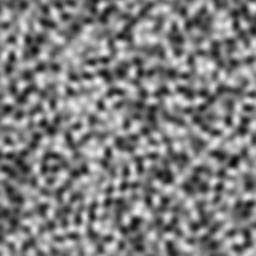
\includegraphics[width=0.3\textwidth]{simplex2}
  \cprotect\caption{\verb|simplex(vec3(x / 16.f, y / 16.f, 0.5f));|}
\end{figure}

\begin{figure}
  \centering
  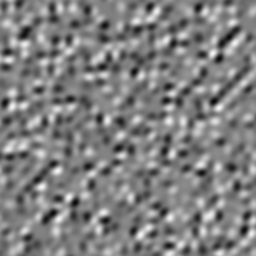
\includegraphics[width=0.3\textwidth]{simplex3}
  \cprotect\caption{\verb|simplex(vec4(x / 16.f, y / 16.f, 0.5f, 0.5f));|}
\end{figure}

\begin{figure}
  \centering
  
\includegraphics[width=0.3\textwidth]{perlin1}
  \cprotect\caption{\verb|perlin(vec2(x / 16.f, y / 16.f));|}
\end{figure}

\begin{figure}
  \centering
  
\includegraphics[width=0.3\textwidth]{perlin2}
  \cprotect\caption{\verb|perlin(vec3(x / 16.f, y / 16.f, 0.5f));|}
\end{figure}

\begin{figure}
  \centering
  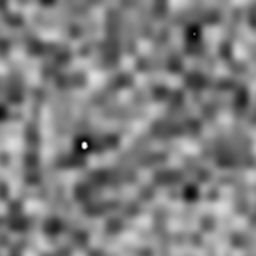
\includegraphics[width=0.3\textwidth]{perlin3}
  \cprotect\caption{\verb|perlin(vec4(x / 16.f, y / 16.f, 0.5f, 0.5f)));|}
\end{figure}

\begin{figure}
  \centering
  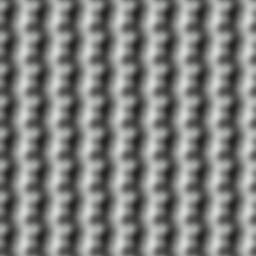
\includegraphics[width=0.3\textwidth]{perlin4}
  \cprotect\caption{\verb|perlin(vec2(x / 16.f, y / 16.f), vec2(2.0f));|}
\end{figure}

\begin{figure}
  \centering
  
\includegraphics[width=0.3\textwidth]{perlin5}
  \cprotect\caption{\verb|perlin(vec3(x / 16.f, y / 16.f, 0.5f), vec3(2.0f));|}
\end{figure}

\begin{figure}
  \centering
  
\includegraphics[width=0.3\textwidth]{perlin6}
  \cprotect\caption{\verb|perlin(vec4(x / 16.f, y / 16.f, vec2(0.5f)), vec4(2.0f));|}
\end{figure}

\subsection{\texttt{GLM\_GTC\_packing}}
\textbf{Header:} \glmheader{gtc/packing}

Convert scalar and vector types to and from packed formats, saving space at the cost of precision. However, packing a value into a format that it was previously unpacked from is \textbf{guaranteed} to be lossless.

\subsection{\texttt{GLM\_GTC\_quaternion}}
\textbf{Header:} \glmheader{gtc/quaternion}

Quaternions and operations upon thereof.

\subsection{\texttt{GLM\_GTC\_random}}
\textbf{Header:} \glmheader{gtc/random}
Probability distributions in up to four dimensions..

\begin{figure}[h]
  \centering
  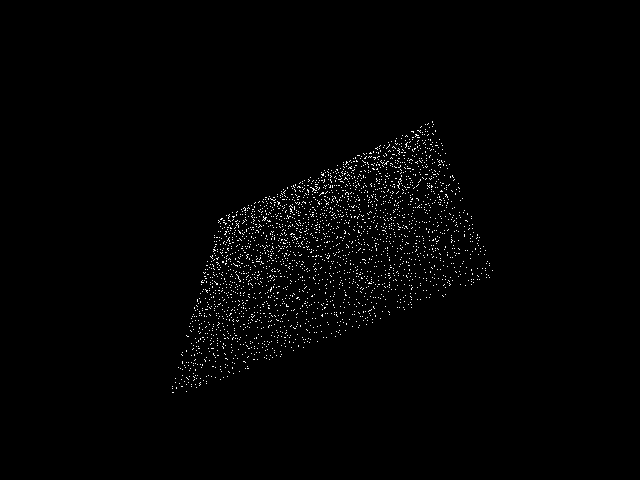
\includegraphics[width=0.5\textwidth]{linearrand}
  \cprotect\caption{\verb|vec4(linearRand(vec2(-1), vec2(1)), 0, 1);|}
\end{figure}

\begin{figure}[h]
  \centering
  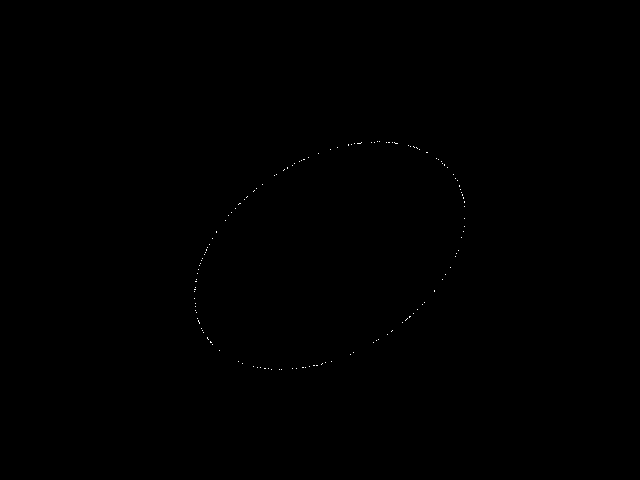
\includegraphics[width=0.5\textwidth]{circularrand}
  \cprotect\caption{\verb|vec4(circularRand(1.0f), 0, 1);|}
\end{figure}

\begin{figure}[h]
  \centering
  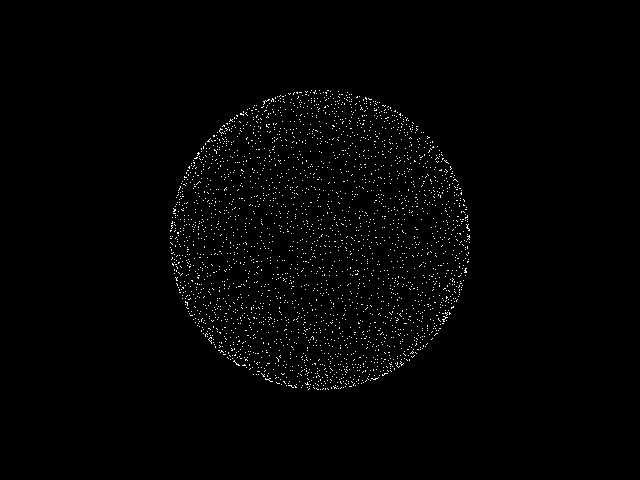
\includegraphics[width=0.5\textwidth]{sphericalrand}
  \cprotect\caption{\verb|vec4(sphericalRand(1.0f), 1);|}
\end{figure}

\begin{figure}[h]
  \centering
  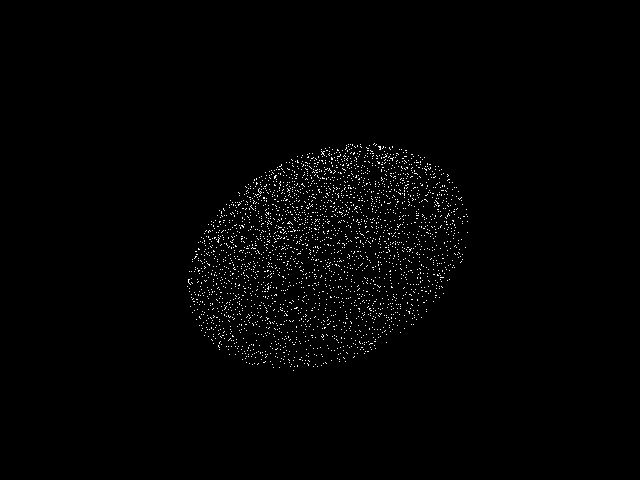
\includegraphics[width=0.5\textwidth]{diskrand}
  \cprotect\caption{\verb|vec4(diskRand(1.0f), 0, 1);|}
\end{figure}

\begin{figure}[h]
  \centering
  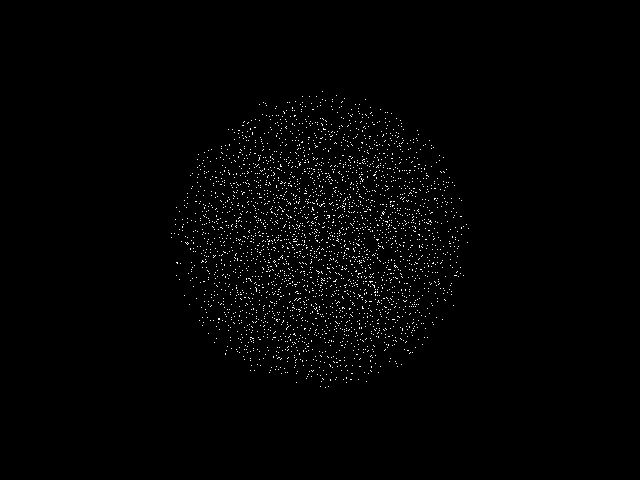
\includegraphics[width=0.5\textwidth]{ballrand}
  \cprotect\caption{\verb|vec4(ballRand(1.0f), 1);|}
\end{figure}

\begin{figure}[h]
  \centering
  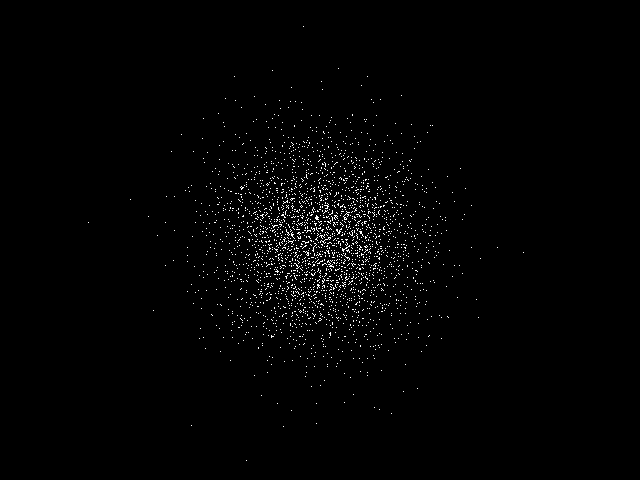
\includegraphics[width=0.5\textwidth]{gaussrand}
  \cprotect\caption{\verb|vec4(gaussRand(vec3(0), vec3(1)), 1);|}
\end{figure}

\subsection{\texttt{GLM\_GTC\_reciprocal}}
\textbf{Header:} \glmheader{gtc/reciprocal}
Reciprocal trigonometric functions (e.g. secant, cosecant, tangent).

\subsection{\texttt{GLM\_GTC\_round}}
\textbf{Header:} \glmheader{gtc/round}
Various rounding operations and common special cases thereof.


\subsection{\texttt{GLM\_GTC\_type\_precision}}
\textbf{Header:} \glmheader{gtc/type\_precision}

Vector and matrix types with defined precisions, e.g. \verb|i8vec4|, which is a 4D vector of signed 8-bit integers.

This extension adds defines to set the default precision of each class of types added, in a manner identical to that described in section \ref{Default Precision}.

Available defines for signed 8-bit integer types (\verb|glm::i8vec|*):

\begin{itemize}
    \item \verb|GLM_PRECISION_LOWP_INT8|: Low precision
    \item \verb|GLM_PRECISION_MEDIUMP_INT8|: Medium precision 
    \item \verb|GLM_PRECISION_HIGHP_INT8|: High precision (default)
\end{itemize}

Available defines for unsigned 8-bit integer types (\verb|glm::u8vec|*):

\begin{itemize}
    \item \verb|GLM_PRECISION_LOWP_UINT8|: Low precision
    \item \verb|GLM_PRECISION_MEDIUMP_UINT8|: Medium precision 
    \item \verb|GLM_PRECISION_HIGHP_UINT8|: High precision (default)
\end{itemize}

Available defines for signed 16-bit integer types (\verb|glm::i16vec|*):

\begin{itemize}
    \item \verb|GLM_PRECISION_LOWP_INT16|: Low precision
    \item \verb|GLM_PRECISION_MEDIUMP_INT16|: Medium precision 
    \item \verb|GLM_PRECISION_HIGHP_INT16|: High precision (default)
\end{itemize}

Available defines for unsigned 16-bit integer types (\verb|glm::u16vec|*):

\begin{itemize}
    \item \verb|GLM_PRECISION_LOWP_UINT16|: Low precision
    \item \verb|GLM_PRECISION_MEDIUMP_UINT16|: Medium precision 
    \item \verb|GLM_PRECISION_HIGHP_UINT16|: High precision (default)
\end{itemize}

Available defines for signed 32-bit integer types (\verb|glm::i32vec|*):

\begin{itemize}
    \item \verb|GLM_PRECISION_LOWP_INT32|: Low precision
    \item \verb|GLM_PRECISION_MEDIUMP_INT32|: Medium precision
    \item \verb|GLM_PRECISION_HIGHP_INT32|: High precision (default)
\end{itemize}

Available defines for unsigned 32-bit integer types (\verb|glm::u32vec|*):

\begin{itemize}
    \item \verb|GLM_PRECISION_LOWP_UINT32|: Low precision
    \item \verb|GLM_PRECISION_MEDIUMP_UINT32|: Medium precision
    \item \verb|GLM_PRECISION_HIGHP_UINT32|: High precision (default)
\end{itemize}

Available defines for signed 64-bit integer types (\verb|glm::i64vec|*):

\begin{itemize}
    \item \verb|GLM_PRECISION_LOWP_INT64|: Low precision
    \item \verb|GLM_PRECISION_MEDIUMP_INT64|: Medium precision
    \item \verb|GLM_PRECISION_HIGHP_INT64|: High precision (default)
\end{itemize}

Available defines for unsigned 64-bit integer types (\verb|glm::u64vec|*):

\begin{itemize}
    \item \verb|GLM_PRECISION_LOWP_UINT64|: Low precision
    \item \verb|GLM_PRECISION_MEDIUMP_UINT64|: Medium precision
    \item \verb|GLM_PRECISION_HIGHP_UINT64|: High precision (default)
\end{itemize}

Available defines for 32-bit floating-point types (\verb|glm::f32vec|*, \verb|glm::f32mat|*, \verb|glm::f32quat|*):

\begin{itemize}
    \item \verb|GLM_PRECISION_LOWP_FLOAT32|: Low precision
    \item \verb|GLM_PRECISION_MEDIUMP_FLOAT32|: Medium precision
    \item \verb|GLM_PRECISION_HIGHP_FLOAT32|: High precision (default)
\end{itemize}

Available defines for 64-bit floating-point types (\verb|glm::f64vec|*, \verb|glm::f64mat|*, \verb|glm::f64quat|*):

\begin{itemize}
    \item \verb|GLM_PRECISION_LOWP_FLOAT64|: Low precision
    \item \verb|GLM_PRECISION_MEDIUMP_FLOAT64|: Medium precision
    \item \verb|GLM_PRECISION_HIGHP_FLOAT64|: High precision (default)
\end{itemize}

\subsection{\texttt{GLM\_GTC\_type\_ptr}}
\textbf{Header:} \glmheader{gtc/type\_ptr}

Facilitate interactions between pointers to raw values (e.g. \verb|float*|) and GLM types (e.g. \verb|mat4|).

This extension defines an overloaded function, \verb|glm::value_ptr|, which returns a pointer to the memory layout of any GLM vector or matrix (\verb|vec3|, \verb|mat4|, etc.).  Matrix types store their values in \textbf{column-major order}.  This is useful for uploading data to matrices or for copying data to buffer objects.

\begin{cppcode}
// GLM_GTC_type_ptr provides a safe solution:
#include <glm/glm.hpp>
#include <glm/gtc/type_ptr.hpp>

void foo()
{
  glm::vec4 v(0.0f);
  glm::mat4 m(1.0f);

  glVertex3fv(glm::value_ptr(v)) 
  glLoadMatrixfv(glm::value_ptr(m));
}
\end{cppcode}

\begin{cppcode}
// Another solution, this one inspired by the STL:
#include <glm/glm.hpp>

void foo()
{
  glm::vec4 v(0.0f);
  glm::mat4 m(1.0f);

  glVertex3fv(&v[0]);
  glLoadMatrixfv(&m[0][0]);
}
\end{cppcode}

Note: It's possible to implement \glfunction{2}{glVertex} and similar functions by defining an implicit cast from GLM types to pointer types.  However, you risk triggering undefined behavior by doing so.

\subsection{\texttt{GLM\_GTC\_ulp}}
\textbf{Header:} \glmheader{gtc/ulp}

Measure a function's accuracy given a reference implementation of it. This extension works on floating-point data and provides results in \href{http://ljk.imag.fr/membres/Carine.Lucas/TPScilab/JMMuller/ulp-toms.pdf}{ULP}.

\subsection{\texttt{GLM\_GTC\_vec1}}
\textbf{Header:} \glmheader{gtc/vec1}

Add *\verb|vec1| types.

\newpage{}

\section{Substituting Deprecated OpenGL Functions}

\subsection{OpenGL Substitutes}

Most fixed-function APIs were deprecated in OpenGL 3.1, and then removed entirely in OpenGL 3.2.  GLM provides substitutes for some of this lost functionality.

\subsubsection{\glfunction{2}{glRotate}}

\begin{cppcode}
glm::mat4 glm::rotate(
  glm::mat4 const & m,
  float angle, 
  glm::vec3 const & axis
);

glm::dmat4 glm::rotate(
  glm::dmat4 const & m,
  double angle, 
  glm::dvec3 const & axis
);
\end{cppcode}

\textbf{Extension:} \verb|GLM_GTC_matrix_transform|

\textbf{Header:} \glmheader{gtc/matrix\_transform}


\subsubsection{\glfunction{2}{glScale}}

\begin{cppcode}
glm::mat4 glm::scale(
  glm::mat4 const & m,
  glm::vec3 const & factors
);

glm::dmat4 glm::scale(
  glm::dmat4 const & m, 
  glm::dvec3 const & factors
);
\end{cppcode}

\textbf{Extension:} \verb|GLM_GTC_matrix_transform|

\textbf{Header:} \glmheader{gtc/matrix\_transform}

\subsubsection{\glfunction{2}{glTranslate}}

\begin{cppcode}
glm::mat4 glm::translate(
  glm::mat4 const & m,
  glm::vec3 const & translation
);

glm::dmat4 glm::translate(
  glm::dmat4 const & m,
  glm::dvec3 const & translation
);
\end{cppcode}

\textbf{Extension:} \verb|GLM_GTC_matrix_transform|

\textbf{Header:} \glmheader{gtc/matrix\_transform}

\subsubsection{\glfunction{2}{glLoadIdentity}}

\begin{cppcode}
glm::mat4(1.0) or glm::mat4();
glm::dmat4(1.0) or glm::dmat4();
\end{cppcode}

\textbf{Extension:} None, part of GLM core

\textbf{Header:} \glmheader{glm}

\subsubsection{\glfunction{2}{glMultMatrix}}

\begin{cppcode}
glm::mat4() * glm::mat4();
glm::dmat4() * glm::dmat4();
\end{cppcode}

\textbf{Extension:} None, part of GLM core

\textbf{Header:} \glmheader{glm}

\subsubsection{\glfunction{2}{glLoadTransposeMatrix}}

\begin{cppcode}
glm::transpose(glm::mat4());
glm::transpose(glm::dmat4());
\end{cppcode}

\textbf{Extension:} None, part of GLM core

\textbf{Header:} \glmheader{glm}

\subsubsection{\glfunction{2}{glMultTransposeMatrix}}

\begin{cppcode}
glm::mat4() * glm::transpose(glm::mat4());
glm::dmat4() * glm::transpose(glm::dmat4());
\end{cppcode}

\textbf{Extension:} None, part of GLM core

\textbf{Header:} \glmheader{glm}


\subsubsection{\glfunction{2}{glFrustum}}

\begin{cppcode}
glm::mat4 glm::frustum(
  float left, float right,
  float bottom, float top,
  float zNear, float zFar
);

glm::dmat4 glm::frustum(
  double left, double right,
  double bottom, double top,
  double zNear, double zFar
);
\end{cppcode}

\textbf{Extension:} \verb|GLM_GTC_matrix_transform|

\textbf{Header:} \glmheader{gtc/matrix\_transform}
 

\subsubsection{\glfunction{2}{glOrtho}}

\begin{cppcode}
glm::mat4 glm::ortho(
  float left, float right, 
  float bottom, float top, 
  float zNear, float zFar
);

glm::dmat4 glm::ortho(
  double left, double right, 
  double bottom, double top, 
  double zNear, double zFar
);
\end{cppcode}

\textbf{Extension:} \verb|GLM_GTC_matrix_transform|

\textbf{Header:} \glmheader{gtc/matrix\_transform}

\subsection{GLU Substitutes}

\subsubsection{\glufunction{gluLookAt}}

\begin{cppcode}
glm::mat4 glm::lookAt(
  glm::vec3 const & eye,
  glm::vec3 const & center,
  glm::vec3 const & up
);

glm::dmat4 glm::lookAt(
  glm::dvec3 const & eye,
  glm::dvec3 const & center,
  glm::dvec3 const & up
);
\end{cppcode}

\textbf{Extension:} \verb|GLM_GTC_matrix_transform|

\textbf{Header:} \glmheader{gtc/matrix\_transform}
 
\subsubsection{\glufunction{gluOrtho2D}}

\begin{cppcode}
glm::mat4 glm::ortho(
  float left, float right, float bottom, float top
);
  
glm::dmat4 glm::ortho(
  double left, double right, double bottom, double top
);
\end{cppcode}

\textbf{Extension:} \verb|GLM_GTC_matrix_transform|

\textbf{Header:} \glmheader{gtc/matrix\_transform}

\subsubsection{\glufunction{gluPerspective}}

\begin{cppcode}
glm::mat4 perspective(
  float fovy, float aspect, float zNear, float zFar
);

glm::dmat4 perspective(
  double fovy, double aspect, double zNear, double zFar
);
\end{cppcode}

Note that in GLM, \verb|fovy| is expressed in \emph{radians}, not degrees.

\textbf{Extension:} \verb|GLM_GTC_matrix_transform|

\textbf{Header:} \glmheader{gtc/matrix\_transform}

\subsubsection{\glufunction{gluPickMatrix}}

\begin{cppcode}
glm::mat4 pickMatrix(
  glm::vec2 const & center, 
  glm::vec2 const & delta, 
  glm::ivec4 const & viewport
);

glm::dmat4 pickMatrix(
  glm::dvec2 const & center, 
  glm::dvec2 const & delta, 
  glm::ivec4 const & viewport
);
\end{cppcode}

\textbf{Extension:} \verb|GLM_GTC_matrix_transform|

\textbf{Header:} \glmheader{gtc/matrix\_transform}

\subsubsection{\glufunction{gluProject}}

\begin{cppcode}
glm::vec3 project(
  glm::vec3 const & obj,
  glm::mat4 const & model,
  glm::mat4 const & proj,
  glm::vec4 const & viewport
);

glm::dvec3 project(
  glm::dvec3 const & obj,
  glm::dmat4 const & model,
  glm::dmat4 const & proj,
  glm::vec4 const & viewport
);
\end{cppcode}

\textbf{Extension:} \verb|GLM_GTC_matrix_transform|

\textbf{Header:} \glmheader{gtc/matrix\_transform}
 
\subsubsection{\glufunction{gluUnProject}}

\begin{cppcode}
glm::vec3 unProject(
  glm::vec3 const & win, 
  glm::mat4 const & model, 
  glm::mat4 const & proj, 
  glm::vec4 const & viewport
);

glm::dvec3 unProject(
  glm::dvec3 const & win, 
  glm::dmat4 const & model, 
  glm::dmat4 const & proj, 
  glm::vec4 const & viewport
);
\end{cppcode}

\textbf{Extension:} \verb|GLM_GTC_matrix_transform|

\textbf{Header:} \glmheader{gtc/matrix\_transform}

\section{Known Issues}
This section reports GLSL features that GLM can't accurately emulate due to language restrictions.

\subsection{The \texttt{not} Function}

The GLSL function \verb|not| is a keyword in C++. To prevent name collisions and ensure a consistent API, the name \verb|not_| (note the underscore) is used instead.

\subsection{Precision Qualifiers}

GLM supports GLSL precision qualifiers through prefixes instead of qualifiers. For example, GLM exposes \verb|lowp_vec4|, \verb|mediump_vec4| and \verb|highp_vec4| as variations of \verb|vec4|.

As in GLSL, GLM precision qualifiers are used to exchange precision for performance.  By default, all types use high precision.

\begin{glslcode}
// Using precision qualifier in GLSL:

ivec3 foo(in vec4 v)
{
  highp vec4 a = v;
  mediump vec4 b = a;
  lowp ivec3 c = ivec3(b);

  returnc;
}
\end{glslcode}

\begin{cppcode}
// Using precision qualifier in GLM:
#include <glm/glm.hpp>

ivec3 foo(const vec4 & v)
{
  highp_vec4 a = v;
  medium_vec4 b = a;
  lowp_ivec3 c = glm::ivec3(b);

  returnc;
}
\end{cppcode}

The syntax for default precision specifications in GLM differs from that in GLSL; for more information, see section \ref{Default Precision}.

\newpage{}

\section{FAQ}

\subsection{Why does GLM follow the GLSL specification?}

Everyone and their dog has their own idea of what should constitute a math library.  The designers of GLSL (the OpenGL ARB) make a living on deciding what should be in its own math library; why not learn from the best and stick to a proven convention?

\subsection{Does GLM actually run GLSL?}

No.  GLM implements a subset of GLSL's functionality.

\subsection{Can GLM be compiled to GLSL (or vice versa)?}

No.  That is not one of GLM's goals.

\subsection{What's the difference between GTX, GTC, and Core?}

GTX extensions are considered \emph{experimental}, and may thus introduce breaking changes without warning (though in practice this doesn't happen often).  GTC extensions are considered \emph{stable}, and are therefore unlikely to introduce radical changes.  Core libraries are based entirely on functionality provided by GLSL, and can safely be relied upon.  The GTX and GTC extension system provides a way to experiment with new GLM functionality, in the hopes of eventually promoting it to a GTC extension.  OpenGL itself is developed in much the same way.

%\subsection{Where can I ask more questions about GLM??}
%
%A good place is the \href{http://www.opengl.org/discussion_boards/ubbthreads.php?ubb=postlist&Board=10&page=1}{OpenGL Toolkits forum} on \href{http://www.opengl.org/}{OpenGL.org}.
%
% TODO: Find the real link

\subsection{Where's the documentation?}

The Doxygen-generated documentation includes a complete list of all extensions available, and can be found right \href{http://glm.g-truc.net/html/index.html}{here}.

\subsection{Should I use \texttt{using namespace glm;}?}

\textbf{Absolutely not!}  GLM uses many common names, such as \verb|any|, \verb|scale|, and \verb|length|.  Haphazardly writing \verb|using namespace glm;| will almost certainly result in name collisions.  Instead, either prefix GLM calls with \verb|glm::|, or pull individual types or functions into your namespace with \verb|using glm::|*, where * is some desired name.

\subsection{Is GLM fast?}

GLM is designed for convenience over performance.  \emph{That being said}, the most frequently-used operations are optimized to the fullest reasonable extent.  Approximations and SIMD-flavored structures are provided as well, in case they're needed.

\subsection{Visual C++ gives me lots of warnings on on warning level \texttt{/W4}.}

You should not have any warnings, even in \verb|/W4| mode. However, if you expect such level for you code, then you should ask for the same level to the compiler by at least disabling the Visual C++ language extensions (\verb|/Za|) which generates warnings when used. If these extensions are enabled, then GLM will take advantage of them and the compiler will generate warnings.

\subsection{Why are some GLM functions vulnerable to division by zero?}

Such behavior is the result of a domain error that follows the precedent set by C and C++. For example, it's a domain error to pass a null vector (all zeroes) to glm::normalize, or even to pass a negative number into \verb|std::sqrt|.

\subsection{What unit does GLM use for angles?}

\textbf{All angles in GLM are expressed in radians unless otherwise noted.}  GLSL does the same thing.  GLU uses degrees, however.  This used to cause a lot of confusion.  For more information, see \href{http://www.g-truc.net/post-0693.html#menu}{here}.

\newpage{}

\section{Code Samples}

\subsection{Compute a Triangle Normal}

\begin{cppcode}
#include <glm/glm.hpp> // vec3 normalize cross

glm::vec3 computeNormal
(
  glm::vec3 const & a, 
  glm::vec3 const & b,
  glm::vec3 const & c
)
{
  return glm::normalize(glm::cross(c - a, b - a));
}
\end{cppcode}

\begin{cppcode}
// A faster (but less accurate) alternative:
#include <glm/glm.hpp> // vec3 cross
#include <glm/gtx/fast_square_root.hpp> // fastNormalize

glm::vec3 computeNormal
(
  glm::vec3 const & a, 
  glm::vec3 const & b,
  glm::vec3 const & c
)
{
  return glm::fastNormalize(glm::cross(c - a, b - a));
}
\end{cppcode}



\subsection{Matrix Transformations}

\begin{cppcode}
#include <glm/glm.hpp> // vec3, vec4, ivec4, mat4
#include <glm/gtc/matrix_transform.hpp> // translate, scale, etc.
#include <glm/gtc/type_ptr.hpp> // value_ptr

using glm::mat4;
using glm::vec3;

void setUniformMVP
(
  GLuint Location, 
  vec3 const & Translate, 
  vec3 const & Rotate
)
{
  mat4 Projection = glm::perspective(45.0f, 4.0f / 3.0f, 0.1f, 100.f);
  mat4 ViewTranslate = glm::translate(
    mat4(1.0f),
    Translate
  );
  mat4 ViewRotateX = glm::rotate(
    ViewTranslate,
    Rotate.y,
    vec3(-1.0f, 0.0f, 0.0f)
  );
  mat4 View = glm::rotate(
    ViewRotateX,
    Rotate.x,
    vec3(0.0f, 1.0f, 0.0f)
  );
  mat4 Model = glm::scale(
    mat4(1.0f),
    vec3(0.5f)
  );
  mat4 MVP = Projection * View * Model;

  glUniformMatrix4fv(Location, 1, GL_FALSE, glm::value_ptr(MVP));
}
\end{cppcode}

\subsection{Vector Types}

\begin{cppcode}
#include <glm/glm.hpp> //vec2
#include <glm/gtc/type_precision.hpp> //hvec2, i8vec2, i32vec2

using glm::vec2;
using glm::hvec2;
using glm::i8vec2;
using glm::i32vec2;

std::size_t const VertexCount = 4;

// Float quad geometry
std::size_t const PositionSizeF32 = VertexCount * sizeof(vec2);
vec2 const PositionDataF32[VertexCount] =
{
  vec2(-1.0f,-1.0f),
  vec2( 1.0f,-1.0f),
  vec2( 1.0f, 1.0f),
  vec2(-1.0f, 1.0f)
};

// Half-float quad geometry
std::size_t const PositionSizeF16 = VertexCount * sizeof(hvec2);
hvec2 const PositionDataF16[VertexCount] =
{
  hvec2(-1.0f, -1.0f),
  hvec2( 1.0f, -1.0f),
  hvec2( 1.0f, 1.0f),
  hvec2(-1.0f, 1.0f)
};

// 8 bits signed integer quad geometry
std::size_t const PositionSizeI8 = VertexCount * sizeof(i8vec2);
i8vec2 const PositionDataI8[VertexCount] =
{
  i8vec2(-1,-1),
  i8vec2( 1,-1),
  i8vec2( 1, 1),
  i8vec2(-1, 1)
};

// 32 bits signed integer quad geometry
std::size_t const PositionSizeI32 = VertexCount * sizeof(i32vec2);
i32vec2 const PositionDataI32[VertexCount] =
{
  i32vec2(-1,-1),
  i32vec2( 1,-1),
  i32vec2( 1, 1),
  i32vec2(-1, 1)
};
\end{cppcode}


\subsection{Lighting}

\begin{cppcode}
#include <glm/glm.hpp> // vec3, normalize, reflect, dot, pow
#include <glm/gtx/random.hpp> // vecRand3

using glm::vec3;
using glm::dot;
using glm::normalize;

// vecRand3, generate a random and equiprobable normalized vec3
vec3 lighting
(
  intersection const & Intersection,
  material const & Material,
  light const & Light,
  vec3 const & View
)
{
  vec3 Color = vec3(0.0f);
  vec3 LightVector = normalize(
    Light.position() - Intersection.globalPosition() +
    glm::vecRand3(0.0f, Light.inaccuracy()
  );
  if(!shadow(
    Intersection.globalPosition(), Light.position(), LightVector)
  )
  {
    float Diffuse = dot(Intersection.normal(), LightVector);
    if(Diffuse <= 0.0f)
      return Color;

    if(Material.isDiffuse())
      Color += Light.color() * Material.diffuse() * Diffuse;

    if(Material.isSpecular())
    {
      vec3 Reflect = glm::reflect(-LightVector, Intersection.normal());
      float Dot = dot(Reflect, View);
      float Base = Dot > 0.0f ? Dot : 0.0f;
      float Specular = glm::pow(Base, Material.exponent());
      Color += Material.specular() * Specular;
    }
  }
  return Color;
}
\end{cppcode}

\newpage{}

\section{References}

\subsection{Official GLM Resources}

\begin{itemize}
  \item \href{http://glm.g-truc.net}{Official website}
  \item \href{https://github.com/g-truc/glm/releases/tag/0.9.7.1}{Latest stable release}
  \item \href{https://github.com/g-truc/glm/archive/master.zip}{HEAD snapshot}
  \item \href{https://github.com/g-truc/glm/issues}{Issue tracker}
  \item \href{http://www.g-truc.net}{G-Truc Creation's Website}
\end{itemize}

\subsection{OpenGL Specifications}

\begin{itemize}
  \item \href{http://www.opengl.org/registry/doc/glspec43.core.20120806.withchanges.pdf}{OpenGL 4.3 core specification}
  \item \href{http://www.opengl.org/registry/doc/GLSLangSpec.4.30.7.diff.pdf}{GLSL 4.30 specification}
  \item \href{http://www.opengl.org/documentation/specs/glu/glu1_3.pdf}{GLU 1.3 specification}
\end{itemize}

\subsection{Projects Using GLM}

\subsubsection{\href{http://outerra.com/}{Outerra}}

3D planetary engine for seamless planet rendering from space down to the surface. Can use arbitrary resolution of elevation data, refining it to centimeter resolution using fractal algorithms.

\begin{center}
  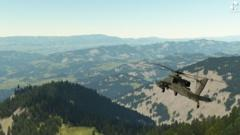
\includegraphics[width=0.4\textwidth]{outerra1}
  
\includegraphics[width=0.4\textwidth]{outerra2}
  
\includegraphics[width=0.4\textwidth]{outerra3}
  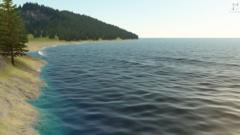
\includegraphics[width=0.4\textwidth]{outerra4}
\end{center}

\subsubsection{\href{https://github.com/mmmovania/opencloth}{opencloth}}

A collection of cloth simulation demos, visualized with OpenGL.

\begin{center}
  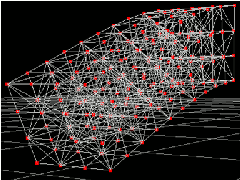
\includegraphics[width=0.35\textwidth]{opencloth1}
  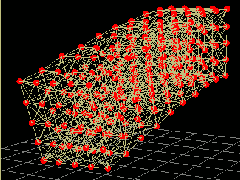
\includegraphics[width=0.35\textwidth]{opencloth2}
  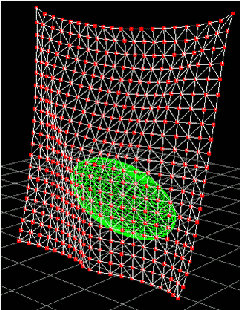
\includegraphics[width=0.35\textwidth]{opencloth3}
  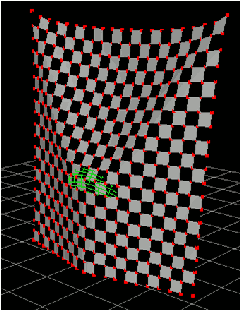
\includegraphics[width=0.35\textwidth]{opencloth4}
\end{center}

\subsubsection{\href{http://www.packtpub.com/opengl-4-0-shading-language-cookbook/book?tag=rk/opengl4-abr1/0811}{OpenGL 4.0 Shading Language Cookbook}}

\begin{wrapfigure}{r}{0.25\textwidth}
  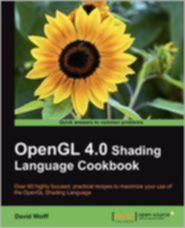
\includegraphics[width=0.25\textwidth, right]{glsl4book}
\end{wrapfigure}

A full set of recipes demonstrating simple and advanced techniques for producing high-quality, real-time 3D graphics using GLSL 4.0.

How to use the OpenGL Shading Language to implement lighting and shading techniques.

Use the new features of GLSL 4.0 including tessellation and geometry shaders.

How to use textures in GLSL as part of a wide variety of techniques from basic texture mapping to deferred shading.

Simple, easy-to-follow examples with GLSL source code, as well as a basic description of the theory behind each technique.

\subsubsection{\href{http://www.leosfortune.com/}{Leo's Forture}}

\begin{wrapfigure}{r}{0.4\textwidth}
  
\includegraphics[width=0.4\textwidth, right]{leosfortune}
  
\includegraphics[width=0.4\textwidth, right]{leosfortune2}
\end{wrapfigure}

Leo's Fortune is a platform adventure game where you hunt down the cunning and mysterious thief that stole your gold. Available on PS4, Xbox One, PC, Mac, iOS and Android.

Beautifully hand-crafted levels bring the story of Leo to life in this epic adventure. 

\say{I just returned home to find all my gold has been stolen! For some devious purpose, the thief has dropped pieces of my gold like breadcrumbs through the woods.}

\say{Despite this pickle of a trap, I am left with no choice but to follow the trail.}

\say{Whatever lies ahead, I must recover my fortune.} ---Leopold

Are you using GLM in a project?  \glmemail{Tell us!}

\subsection{OpenGL Tutorials using GLM}

\begin{itemize}
  \item \href{http://www.g-truc.net/project-0026.html#menu}{The OpenGL Samples Pack}: Examples that demonstrate OpenGL's many features
  \item \href{http://www.arcsynthesis.org/gltut/}{Learning Modern 3D Graphics Programming}: A great OpenGL tutorial by Jason L. McKesson
  \item \href{http://blog.nobel-joergensen.com/2011/04/02/glm-brilliant-math-library-for-opengl/}{Morten Nobel-Jørgensen's review} and \href{https://github.com/mortennobel/RenderE}{OpenGL renderer} 
  \item \href{http://www.swiftless.com/opengltuts.html}{Swiftless' OpenGL tutorial} by Donald Urquhart
  \item \href{http://rastergrid.com/blog/}{Rastergrid}: Technical articles (with companion programs) by Daniel Rákos
  \item \href{http://www.opengl-tutorial.org}{OpenGL Tutorial}: OpenGL tutorials
  \item \href{http://en.wikibooks.org/wiki/OpenGL_Programming}{OpenGL Programming on Wikibooks}: For beginners just discovering OpenGL
  \item \href{http://3dgep.com/}{3D Game Engine Programming}: 3D game engine programming techniques
  \item \href{http://www.gametutorials.com/opengl-4-matrices-and-glm/}{Game Tutorials}: Graphics and game programming tutorials 
  \item \href{https://open.gl/}{open.gl}: An OpenGL tutorial
  \item \href{http://www.c-jump.com/bcc/common/Talk3/Math/GLM/GLM.html}{c-jump}: A GLM tutorial
  \item \href{http://learnopengl.com/}{Learn OpenGL}: An OpenGL tutorial
\end{itemize}

Are you using GLM in a tutorial?  \glmemail{Tell us!}


\subsection{Alternatives to GLM}

\begin{itemize}
  \item \href{http://cmldev.net/}{CML}: The CML (Configurable Math Library) is a free C++ math library for games and graphics.
  \item \href{http://eigen.tuxfamily.org/}{Eigen}: A more heavy weight math library for general linear algebra in C++.
  \item \href{http://glhlib.sourceforge.net/}{glhlib}: A much more than glu C library.
\end{itemize}

Are you using or developing an alternative to GLM?  \glmemail{Tell us!}

\subsection{Acknowledgements}

GLM is developed and maintained by \href{http://www.g-truc.net}{Christophe Riccio}, but relies on the support of its many contributors to stay great.

Special thanks to:

\begin{itemize}
  \item Ashima Arts and Stefan Gustavson for their work on \href{https://github.com/ashima/webgl-noise}{webgl-noise}, which which is the base of \verb|GLM_GTC_noise|.
  \item \href{http://athile.net/library/wiki/index.php?title=Athile_Technologies}{Arthur Winters} for contributing to the swizzle operator implementation.
  \item Joshua Smith and Christoph Schied for their contributions to the swizzle operator implementation.
  \item Guillaume Chevallereau for providing and maintaining the \href{http://my.cdash.org/index.php?project=GLM}{nightly build system}.
  \item Ghenadii Ursachi for \verb|GLM_GTX_matrix_interpolation|.
  \item Mathieu Roumillac for providing some implementation ideas.
  \item \href{http://www.zeuscmd.com/}{Grant James} for non-square matrix multiplication (e.g. \verb|mat3 * 3x2|)
  \item GLM's users!  Without you, there is no GLM!
\end{itemize}

\subsection{Quotes from the web}

\say{I am also going to make use of boost for its time framework and the matrix library GLM, a GL Shader-like Math library for C++. A little advertise for the latter which has a nice design and is useful since matrices have been removed from the latest OpenGL versions.}
\begin{flushright}
---\href{http://www.codexperiments.com/android/2010/10/android-sdk-ndk-part-4-the-silver-bullet-of-android/}{Code Xperiments}
\end{flushright}

\say{OpenGL Mathematics Library (GLM): Used for vector classes, quaternion classes, matrix classes and math operations that are suited for OpenGL applications.}
\begin{flushright}
---\href{http://3dgep.com/?p=1116}{Jeremiah van Oosten}
\end{flushright}

\say{Today I ported my code base from my own small linear algebra library to GLM, a GLSL-style vector library for C++. The transition went smoothly.}
\begin{flushright}
---\href{http://devel.leonard-ritter.com/2011/08/planning-sparse-voxel-octrees.html}{Leonard Ritter}
\end{flushright}

\say{A more clever approach is to use a math library like GLM instead. I wish someone had showed me this library a few years ago.}
\begin{flushright}
---\href{http://blog.nobel-joergensen.com/2011/04/02/glm-brilliant-math-library-for-opengl/}{Morten Nobel-Jørgensen}
\end{flushright}

\end{document}